% 这部分专门用来介绍meson系统

% \usepackage{listings, listings-rust} 第二个宏包是需要添加的,因为原本的listings不支持rust
% \usepackage[dvipsnames]{xcolor}
% \setmonofont{DejaVu Sans Mono} 这个是用来显示下面的一个文件树状结构的

\subsection{Meson构建系统}
\subsubsection{Meson介绍}
\indent 
Meson是一个开源构建系统\cite{meson_system},其设计目标是提供极高的构建速度和尽可能友好的用户体验。Meson采用声明式配置,避免了传统构建系统复杂的配置过程,从而减少开发者在编写或调试构建定义上所耗费的时间。此外,Meson采用Ninja作为底层构建工具,使得构建过程高效且快速,显著减少了编译启动时的等待时间。

\indent 作为一个现代化的构建系统\cite{Wiki_Meson},Meson 具备原生的Rust支持,可以直接调用 \texttt{rustc} 或 \texttt{Cargo} 进行构建,并能自动生成Ninja构建文件。其语法简洁且类似于Python,使得开发者更易上手,同时也降低了多语言项目的集成成本。与传统的 SCons、CMake 等构建系统相比,Meson的构建速度更快,尤其适用于 CI/CD 持续集成环境。此外,Meson 的轻量级特性使其在嵌入式开发场景下表现出色\cite{embedded},不仅减少了系统开销,还提供了对多架构和交叉编译的良好支持\cite{RioTian}。

\indent 在嵌入式系统开发中,构建系统的选择至关重要。Meson 通过其简洁的配置方式、强大的多语言支持以及卓越的性能,成为嵌入式开发者值得考虑的方案。无论是针对资源受限的设备进行优化,还是实现高效的固件编译流程,Meson 都能提供可靠的支持。

\subsubsection{配置meson系统环境}
\indent 我选择在WSL的Ubuntu22.04系统中配置meson系统。Meson需要python环境和Ninja环境\cite{meson_install},所以首先安装
\begin{lstlisting}[
    language=bash,
    basicstyle=\ttfamily\small,
    keywordstyle=\color{blue},
    commentstyle=\color{green},
    stringstyle=\color{red},
    numbers=none,
    numberstyle=\tiny\color{gray},
    stepnumber=1,
    numbersep=5pt,
    tabsize=2,
    frame=lines,
    captionpos=b
]
sudo apt-get install python3 python3-pip ninja-build
pip3 install --user meson # install meson through pip
\end{lstlisting}

这里显示安装成功,如果使用meson --version,发现仍然检测不到meson,这里还需要继续设置环境变量
\begin{lstlisting}[
    language=bash,
    basicstyle=\ttfamily\small,
    keywordstyle=\color{blue},
    commentstyle=\color{green},
    stringstyle=\color{red},
    numbers=none,
    numberstyle=\tiny\color{gray},
    stepnumber=1,
    numbersep=5pt,
    tabsize=2,
    frame=lines,
    captionpos=b
]
echo 'export PATH=$HOME/.local/bin:$PATH' >> ~/.bashrc
source ~/.bashrc
meson --version
\end{lstlisting}
到这里应该能正确输出Meson的版本,即已经正确安装Meson构建系统。下面为了了测试在meson系统上联合编译Rust和C语言的可行性,我创建了一个简单的Meson项目来进行测试。首先需要安装一些必要的编译链工具和库文件,以便于支持交叉编译和运行。可以使用以下命令来安装这些工具:

\begin{lstlisting}[
    language=bash,
    basicstyle=\ttfamily\small,
    keywordstyle=\color{blue},
    commentstyle=\color{green},
    stringstyle=\color{red},
    numbers=none,
    numberstyle=\tiny\color{gray},
    stepnumber=1,
    numbersep=5pt,
    tabsize=2,
    frame=lines,
    captionpos=b
]
snap install rustup --classic
sudo apt-get install gcc-arm-linux-gnueabihf
sudo apt install gcc-arm-none-eabi
sudo apt install g++-arm-linux-gnueabihf
rustup target add arm-unknown-linux-gnueabihf
apt install qemu-user
curl --proto '=https' --tlsv1.2 -sSf https://sh.rustup.rs | sh
rustup target add arm-unknown-linux-gnueabihf
\end{lstlisting}

\subsubsection{创建Meson测试项目}
\indent 创建一个新的目录来存放Meson项目,并在该目录下创建以下文件结构:
\begin{verbatim}
├── meson.build
├── my_cross_file.txt
├── rust
│   └── rust_lib.rs
├── rustc_arm.sh
└── src
    └── main.c
\end{verbatim}

这里的c语言代码文件需要一些特殊的处理,如图\ref{c_test}
\begin{figure}[!htpb]
    \centering
    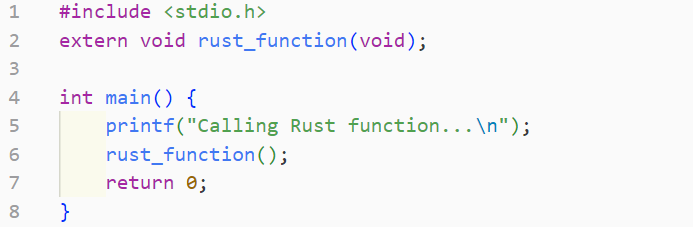
\includegraphics[width=0.8\textwidth]{assets/c_test.png}
    \caption{C代码测试文件}
    \label{c_test}
\end{figure}

Rust代码中需要声明C语言函数的接口,以便于C语言调用Rust函数。Rust函数需使用\#[no\_mangle]和extern "C"属性,确保函数名不被修饰并符合C调用约定,如图\ref{rust_test}所示。
\begin{figure}[!htpb]
    \centering
    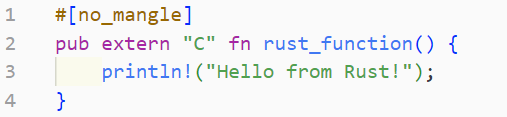
\includegraphics[width=0.8\textwidth]{assets/rust_test.png}
    \caption{Rust代码测试文件}
    \label{rust_test}
\end{figure}

\indent \texttt{meson.build}是Meson构建系统的核心配置文件,定义了项目的构建规则和依赖关系。这里只需要一句简单的\texttt{project
('test\_cross\_com\\
pilation', 'c', 'rust')},就能够实现项目的交叉编译,这是与其它构建系统相比的巨大优势。
\indent 在进行C语言和Rust语言的交叉编译时,还需要额外的配置文件和工具:
\begin{itemize}
\item \texttt{my\_cross\_file.txt}是交叉编译配置文件,指定了目标平台、编译器和系统库等信息,确保 Meson 在构建时能够正确使用交叉工具链。
\item \texttt{rust\_lib.rs} 是Rust语言编写的库文件,其中定义了供C语言调用的Rust函数,使用 \texttt{\#[no\_mangle]}以保证函数符号不会被修改。
\item \texttt{src/main.c} 是C语言编写的主程序文件,负责调用Rust代码,并进行必要的数据转换。
\item \texttt{rustc\_arm.sh}作为 Rust 编译器 \texttt{rustc}的包装器,确保 Rust 代码能正确编译为目标架构的二进制文件。
\end{itemize}

\indent 在使用Meson进行交叉编译时,首先需要使用 \texttt{meson setup}指定交叉编译配置文件,例如:
\begin{verbatim}
meson setup build --cross-file my_cross_file.txt
ninja -C build
\end{verbatim}
这样,Meson 将自动检测并配置C和Rust的交叉编译工具链,最终生成适用于目标平台的可执行文件。

\begin{lstlisting}[
    language=bash,
    basicstyle=\ttfamily\small,
    keywordstyle=\color{blue},
    commentstyle=\color{green},
    stringstyle=\color{red},
    tabsize=2,
    frame=lines,
    captionpos=b,
    breaklines=true
]
project('test_cross_compilation', 'c', 'rust')

# compile Rust static library
rust_lib = custom_target('rust_lib',
    input: 'rust/rust_lib.rs',
    output: 'librust_lib.a',
    command: ['/home/courses/osh/project/rustc_arm.sh', '--crate-type=staticlib', '-o', '@OUTPUT@', '@INPUT@']
)

# compile c executable file, and link it to Rust library
c_exe = executable('myprogram', 'src/main.c', link_with: rust_lib)
\end{lstlisting}
\indent rust\_lib 通过static\_library函数构建的Rust静态库,默认情况下使用Rust 
\space ABP(Application Binary Interface)来链接Rust和C代码。custom\_target函数用于定义一个自定义的构建目标,这里我们指定了Rust源文件和编译命令。最后,executable函数用于编译C语言的可执行文件,并将Rust静态库链接到可执行文件中。但是因为Meson在处理Rust和的缓和构建的时候,对目标类型有严格的限制,而Rust \space ABI的静态库只能与Rust目标链接,不能链接C目标,所以我们需要使用custom\_target函数来创建一个自定义的构建目标,将Rust静态库编译为C语言可执行文件。

\indent 接下来是交叉编译的关键步骤,需要创建一个交叉编译配置文件\\\texttt
{my\_cross\_file.txt},该文件指定了目标平台、编译器和系统库等信息。图\ref
{cross_set}是我们在测试时使用的配置。
\begin{figure}[!htpb]
    \centering
    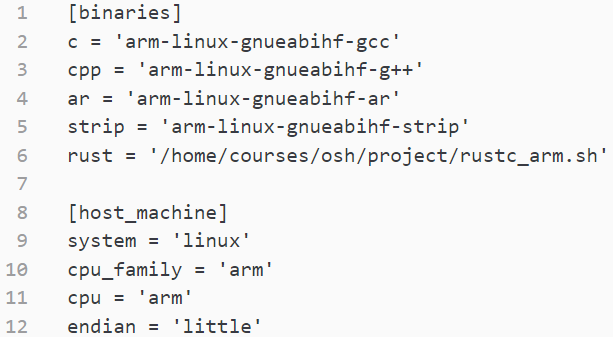
\includegraphics[width=0.8\linewidth]{assets/cross_set.png}
    \caption{交叉编译配置文件}
    \label{cross_set}
\end{figure}

\begin{itemize}
    \item \textbf{C 语言编译器}:使用 \texttt{arm-linux-gnueabihf-gcc} 进行 C 语言的交叉编译。
    \item \textbf{C++ 语言编译器}:使用 \texttt{arm-linux-gnueabihf-g++} 进行 C++ 代码编译。
    \item \textbf{静态库管理}:\texttt{arm-linux-gnueabihf-ar} 用于管理静态库。
    \item \textbf{去除调试信息}:\texttt{arm-linux-gnueabihf-strip} 用于精简二进制文件。
    \item \textbf{Rust 交叉编译}:由于 Rust 交叉编译需要额外的配置,使用脚本 \texttt{rustc\_arm.sh} 代理 \texttt{rustc}。
    \end{itemize}
    
    \subsection{目标主机架构}
    \begin{itemize}
    \item \textbf{system = 'linux'} :目标系统为 Linux。
    \item \textbf{cpu\_family = 'arm'} :目标 CPU 架构为 ARM。
    \item \textbf{endian = 'little'} :采用小端存储格式。
    \end{itemize}

\indent 执行下面的指令可以构建这个项目并编译。这里Meson本身并不直接编译代码,而是生
成构建文件并交给Ninja来完成具体工作。最后使用qume测试生成的可执行文件。
\begin{lstlisting}[
    language=bash,
    basicstyle=\ttfamily\small,
    keywordstyle=\color{blue},
    commentstyle=\color{green},
    stringstyle=\color{red},
    tabsize=2,
    frame=lines,
    captionpos=b,
    caption={配置和运行Meson项目}
]
# start
meson setup build --cross-file my_cross_file.txt
meson compile -C build
# test on qume
qemu-arm -L /usr/arm-linux-gnueabihf build/myprogram
\end{lstlisting}
如图\ref{cross_compilation}所示,成功运行了C语言调用Rust函数的测试程序
\begin{figure}[!htpb]
    \centering
    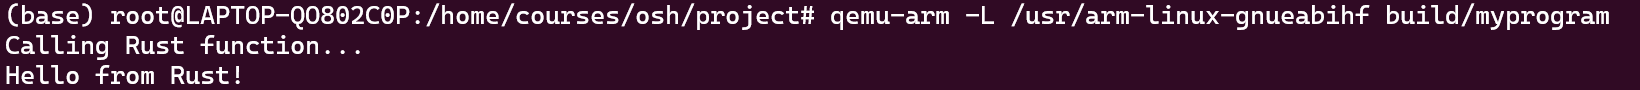
\includegraphics[width=1\linewidth]{assets/meson_result.png}
    \caption{交叉编译测试结果}
    \label{cross_compilation}
\end{figure}
